\documentclass{beamer}
\usepackage[utf8]{inputenc}
\usepackage{graphicx, epsfig}
\usepackage{amsmath,mathrsfs,amsfonts,amssymb}
%\usepackage{subfig}
\usepackage{floatflt}
\usepackage{epic,ecltree}
\usepackage{mathtext}
\usepackage{fancybox}
\usepackage{fancyhdr}
\usepackage{multirow}
\usepackage{enumerate}
\usepackage{epstopdf}
\usepackage{multicol}
\usepackage{algorithm}
\usepackage[noend]{algorithmic}
\usepackage{tikz}
\usepackage{blindtext}
\usetheme{default}%{Singapore}%{Warsaw}%{Warsaw}%{Darmstadt}
\usecolortheme{default}
\setbeamerfont{title}{size=\Huge}
\setbeamertemplate{footline}[page number]{}


\makeatletter
\newcommand\HUGE{\@setfontsize\Huge{35}{40}}
\makeatother    

\setbeamerfont{title}{size=\HUGE}
\beamertemplatenavigationsymbolsempty

% latin bold lower
\newcommand{\ba}{\mathbf{a}} 
\newcommand{\bc}{\mathbf{c}} 
\newcommand{\be}{\mathbf{e}} 
\newcommand{\bh}{\mathbf{h}} 
\newcommand{\bp}{\mathbf{p}} 
\newcommand{\bt}{\mathbf{t}} 
\newcommand{\bs}{\mathbf{s}} 
\newcommand{\bu}{\mathbf{u}} 
\newcommand{\bv}{\mathbf{v}} 
\newcommand{\bw}{\mathbf{w}} 
\newcommand{\bx}{\mathbf{x}} 
\newcommand{\by}{\mathbf{y}} 
\newcommand{\bz}{\mathbf{z}} 

% latin bold upper
\newcommand{\bA}{\mathbf{A}} 
\newcommand{\bB}{\mathbf{B}} 
\newcommand{\bC}{\mathbf{C}} 
\newcommand{\bI}{\mathbf{I}} 
\newcommand{\bL}{\mathbf{L}} 
\newcommand{\bM}{\mathbf{M}} 
\newcommand{\bQ}{\mathbf{Q}} 
\newcommand{\bT}{\mathbf{T}} 
\newcommand{\bU}{\mathbf{U}} 
\newcommand{\bV}{\mathbf{V}} 
\newcommand{\bW}{\mathbf{W}} 
\newcommand{\bX}{\mathbf{X}} 
\newcommand{\bY}{\mathbf{Y}} 
\newcommand{\bZ}{\mathbf{Z}} 

% latin cal upper
\newcommand{\cG}{\mathcal{G}} 
\newcommand{\cL}{\mathcal{L}} 
\newcommand{\cN}{\mathcal{N}} 
\newcommand{\cS}{\mathcal{S}} 
\newcommand{\cT}{\mathcal{T}} 
\newcommand{\cW}{\mathcal{W}} 
\newcommand{\cX}{\mathcal{X}} 
\newcommand{\cZ}{\mathcal{Z}} 

% latin bb upper
\newcommand{\bbE}{\mathbb{E}} 
\newcommand{\bbI}{\mathbb{I}} 
\newcommand{\bbP}{\mathbb{P}} 
\newcommand{\bbR}{\mathbb{R}} 

% greek bold lower
\newcommand{\bepsilon}{\boldsymbol{\epsilon}} 
\newcommand{\btheta}{\boldsymbol{\theta}} 
\newcommand{\blambda}{\boldsymbol{\lambda}} 
\newcommand{\bpi}{\boldsymbol{\pi}} 
\newcommand{\bmu}{\boldsymbol{\mu}} 
\newcommand{\bsigma}{\boldsymbol{\sigma}} 
\newcommand{\bphi}{\boldsymbol{\phi}} 

% greek bold upper
\newcommand{\bSigma}{\boldsymbol{\Sigma}} 

\DeclareMathOperator*{\argmin}{arg\,min}
\DeclareMathOperator*{\argmax}{arg\,max}

\newcommand{\createdgmtitle}[1]{\title[\hbox to 56mm{Deep Generative Models  \hfill\insertframenumber\,/\,\inserttotalframenumber}]
	{\vspace{1.5cm} \\ Deep Generative Models \\ {\Huge Lecture #1}}
	\author{Roman Isachenko}
	\institute{
	Moscow Institute of Physics and Technology
	} 
	\date{Autumn, 2021}
}

\newcommand\myfootnote[1]{%
  \tikz[remember picture,overlay]
  \draw (current page.south west) +(1in + \oddsidemargin,0.5em)
  node[anchor=south west,inner sep=0pt]{\parbox{\textwidth}{%
      \rlap{\rule{10em}{0.4pt}}\raggedright\scriptsize \textit{#1}}};}

\newcommand\myfootnotewithlink[2]{%
  \tikz[remember picture,overlay]
  \draw (current page.south west) +(1in + \oddsidemargin,0.5em)
  node[anchor=south west,inner sep=0pt]{\parbox{\textwidth}{%
      \rlap{\rule{10em}{0.4pt}}\raggedright\scriptsize\href{#1}{\textit{#2}}}};}
\createdgmtitle{8}
%--------------------------------------------------------------------------------
\begin{document}
%--------------------------------------------------------------------------------
\begin{frame}[noframenumbering,plain]
%\thispagestyle{empty}
\titlepage
\end{frame}
%=======
\begin{frame}{Flows in VAE posterior}
	Apply a sequence of transformations to the random variable
	\[
	\bz_0 \sim q(\bz | \bx, \bphi) = \mathcal{N}(\bz| \bmu_{\bphi}(\bx), \bsigma^2_{\bphi}(\bx)).
	\]
	Let $q(\bz | \bx, \bphi)$ (VAE encoder) be a base distribution for a flow model.
	
	\begin{block}{Flow model in latent space}
		\vspace{-0.3cm}
		\[
			\log q(\bz^* | \bx, \bphi, \blambda) = \log q(\bz | \bx, \bphi) + \log \det \left | \frac{\partial f(\bz, \blambda)}{\partial \bz}\right|
		\]
		\[
			\bz^* = f(\bz, \blambda) = g^{-1}(\bz, \blambda)
		\]
	\end{block}
	Here $f(\bz, \blambda)$ is a flow model (e.g. stack of planar/coupling layers) parameterized by $\blambda$.
	
	
	Let use $q(\bz^* | \bx, \bphi, \blambda)$ as a variational distribution. Here $\bphi$~-- encoder parameters, $\blambda$~-- flow parameters.
	
	\myfootnotewithlink{https://arxiv.org/abs/1505.05770}{Rezende D. J., Mohamed S. Variational Inference with Normalizing Flows, 2015} 
\end{frame}
%=======
\begin{frame}{Flows-based VAE posterior}
	\begin{itemize}
		\item Encoder outputs base distribution $q(\bz | \bx, \bphi)$.
		\item Flow model $\bz^* = f(\bz, \blambda)$ transforms the base distribution $q(\bz | \bx, \bphi)$ to the distribution $q(\bz^* | \bx, \bphi, \blambda)$.
		\item Distribution $q(\bz^* | \bx, \bphi, \blambda)$ is used as a variational distribution for ELBO maximization.
	\end{itemize}
	
	\begin{block}{Flow model in latent space}
		\vspace{-0.3cm}
		\[
			\log q(\bz^* | \bx, \bphi, \blambda) = \log q(\bz | \bx, \bphi) + \log \det \left | \frac{\partial f(\bz, \blambda)}{\partial \bz}\right|
		\]
		\vspace{-0.3cm}
	\end{block}
	\begin{block}{ELBO with flow-based VAE posterior}
		\vspace{-0.5cm}
		\begin{align*}
			\mathcal{L} (\bphi, \btheta, \blambda)  
			&= \bbE_{q(\bz^* | \bx, \bphi, \blambda)} \bigl[\log p(\bx, \bz^* | \btheta) - \log q(\bz^*| \bx, \bphi, \blambda) \bigr] \\ 
			&=  \bbE_{q(\bz^* | \bx, \bphi, \blambda)} \log p(\bx | \bz^*, \btheta) - KL (q(\bz^* | \bx, \bphi, \blambda) || p(\bz^*)).
		\end{align*}
		\vspace{-0.4cm}
	\end{block}
	The second term in ELBO is reverse KL divergence. Planar flows was originally proposed for variational inference in VAE.
	
	\myfootnotewithlink{https://arxiv.org/abs/1505.05770}{Rezende D. J., Mohamed S. Variational Inference with Normalizing Flows, 2015} 
\end{frame}
%=======
\begin{frame}{Flows-based VAE posterior}
	
	\begin{block}{Flow model in latent space}
		\vspace{-0.3cm}
		\[
			\log q(\bz^* | \bx, \bphi, \blambda) = \log q(\bz | \bx, \bphi) + \log \det \left | \frac{\partial f(\bz, \blambda)}{\partial \bz}\right|
		\]
		\vspace{-0.3cm}
	\end{block}
	\begin{block}{ELBO objective}
		\vspace{-0.5cm}
		\begin{multline*}
			\mathcal{L} (\bphi, \btheta, \blambda)  
			= \mathbb{E}_{q(\bz^* | \bx, \bphi, \blambda)} \bigl[\log p(\bx, \bz^* | \btheta) - \log q(\bz^*| \bx, \bphi, \blambda) \bigr] = \\
			= \mathbb{E}_{q(\bz | \bx, \bphi)} \left. \bigl[\log p(\bx, \bz^* | \btheta) - \log q(\bz^*| \bx, \bphi, \blambda) \bigr]\right|_{\bz^* = f(\bz, \blambda)} = \\
			= \mathbb{E}_{q(\bz | \bx, \bphi)} \bigg[\log p(\bx, \bz^* | \btheta) -  \log q(\bz | \bx, \bphi ) + \log \left| \det \left( \frac{\partial f(\bz, \blambda)}{\partial \bz} \right) \right| \bigg].
		\end{multline*}
	\end{block}
	\begin{itemize}
		\item Obtain samples $\bz$ from the encoder $q(\bz | \bx, \bphi)$.
		\item Apply flow model $\bz^* = f(\bz, \blambda)$.
		\item Compute likelihood for $\bz^*$ using the decoder, base distribution for $\bz^*$ and the Jacobian.
	\end{itemize}
	\myfootnotewithlink{https://arxiv.org/abs/1505.05770}{Rezende D. J., Mohamed S. Variational Inference with Normalizing Flows, 2015} 
\end{frame}
%=======
\begin{frame}{Inverse autoregressive flow (IAF)}
	\vspace{-0.3cm}
	\begin{align*}
		\bx &= g(\bz, \btheta) \quad \Rightarrow \quad x_i = \tilde{\sigma}_i (\bz_{1:i-1}) \cdot z_i + \tilde{\mu}_i(\bz_{1:i-1}). \\
		\bz &= f(\bx, \btheta) \quad \Rightarrow \quad z_i = \left(x_i - \tilde{\mu}_i(\bz_{1:i-1}) \right) \cdot \frac{1}{\tilde{\sigma}_i (\bz_{1:i-1})}.
	\end{align*}
	\vspace{-0.5cm}
	\begin{block}{Reverse KL for flow model}
  		\vspace{-0.5cm}
		\[
			KL(p || \pi)  = \bbE_{p(\bz)} \left[  \log p(\bz) - \log \left|\det \left( \frac{\partial g(\bz, \btheta)}{\partial \bz} \right) \right| - \log \pi(g(\bz, \btheta)) \right]
		\]
		\vspace{-0.3cm}
	\end{block}
	\begin{itemize}
	\item We don’t need to think about computing the function $f(\bx, \btheta)$.
	\item Inverse autoregressive flow is a natural choice for using flows in VAE:
	\end{itemize}
	\vspace{-0.3cm}
	\begin{align*}
		\bz &= \bsigma(\bx) \odot \bepsilon + \bmu(\bx), \quad \bepsilon \sim \mathcal{N}(0, 1); \quad  \sim q(\bz | \bx, \bphi). \\
		\bz_k &= \tilde{\bsigma}_k(\bz_{k - 1}) \odot \bz_{k-1} + \tilde{\bmu}_k(\bz_{k - 1}), \quad k \geq 1; \quad  \sim q_k(\bz_k | \bx, \bphi, \{\blambda_j\}_{j=1}^k).
	\end{align*}
	\myfootnotewithlink{https://arxiv.org/abs/1606.04934}{Kingma D. P. et al. Improving Variational Inference with Inverse Autoregressive Flow, 2016} 
\end{frame}
%=======
\begin{frame}{Inverse autoregressive flow (IAF)}
	\begin{figure}
		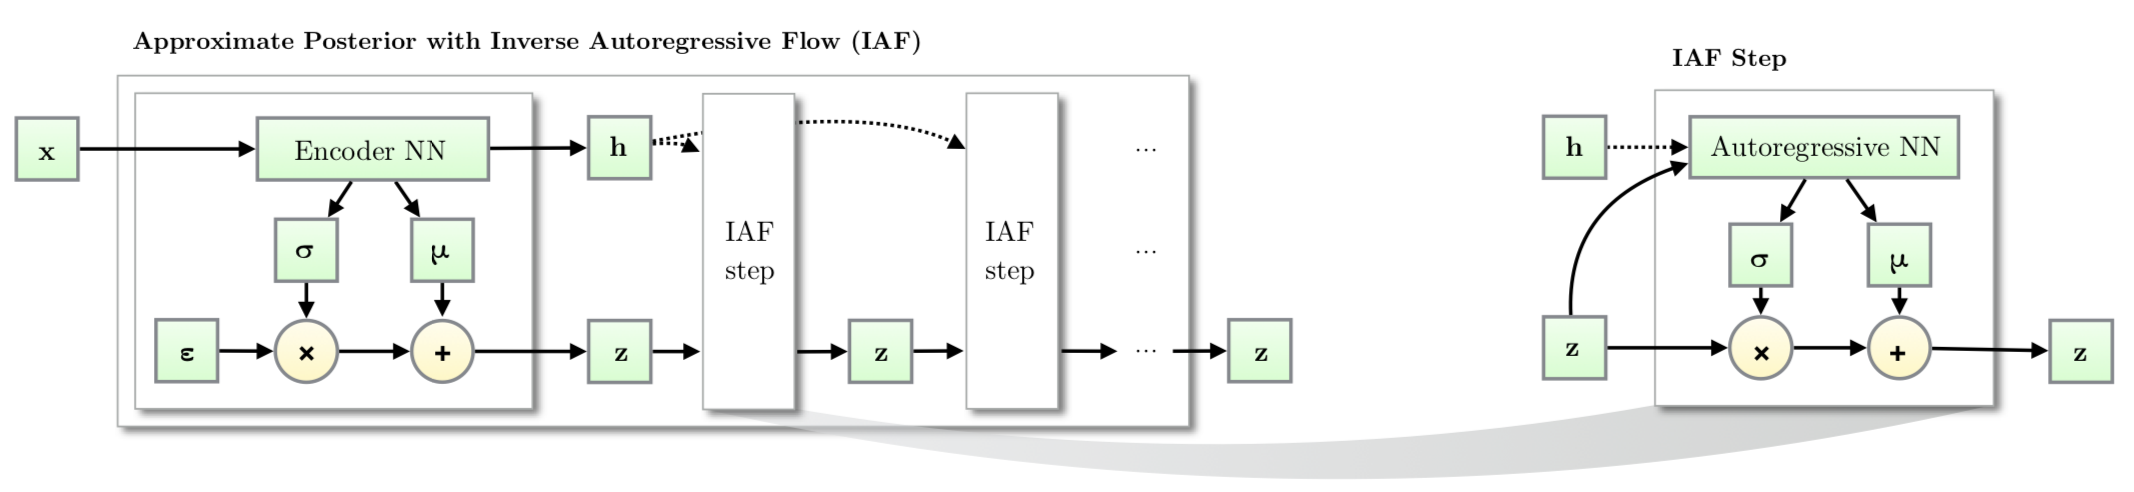
\includegraphics[width=\linewidth]{figs/iaf2.png}
	\end{figure}
	\begin{figure}
		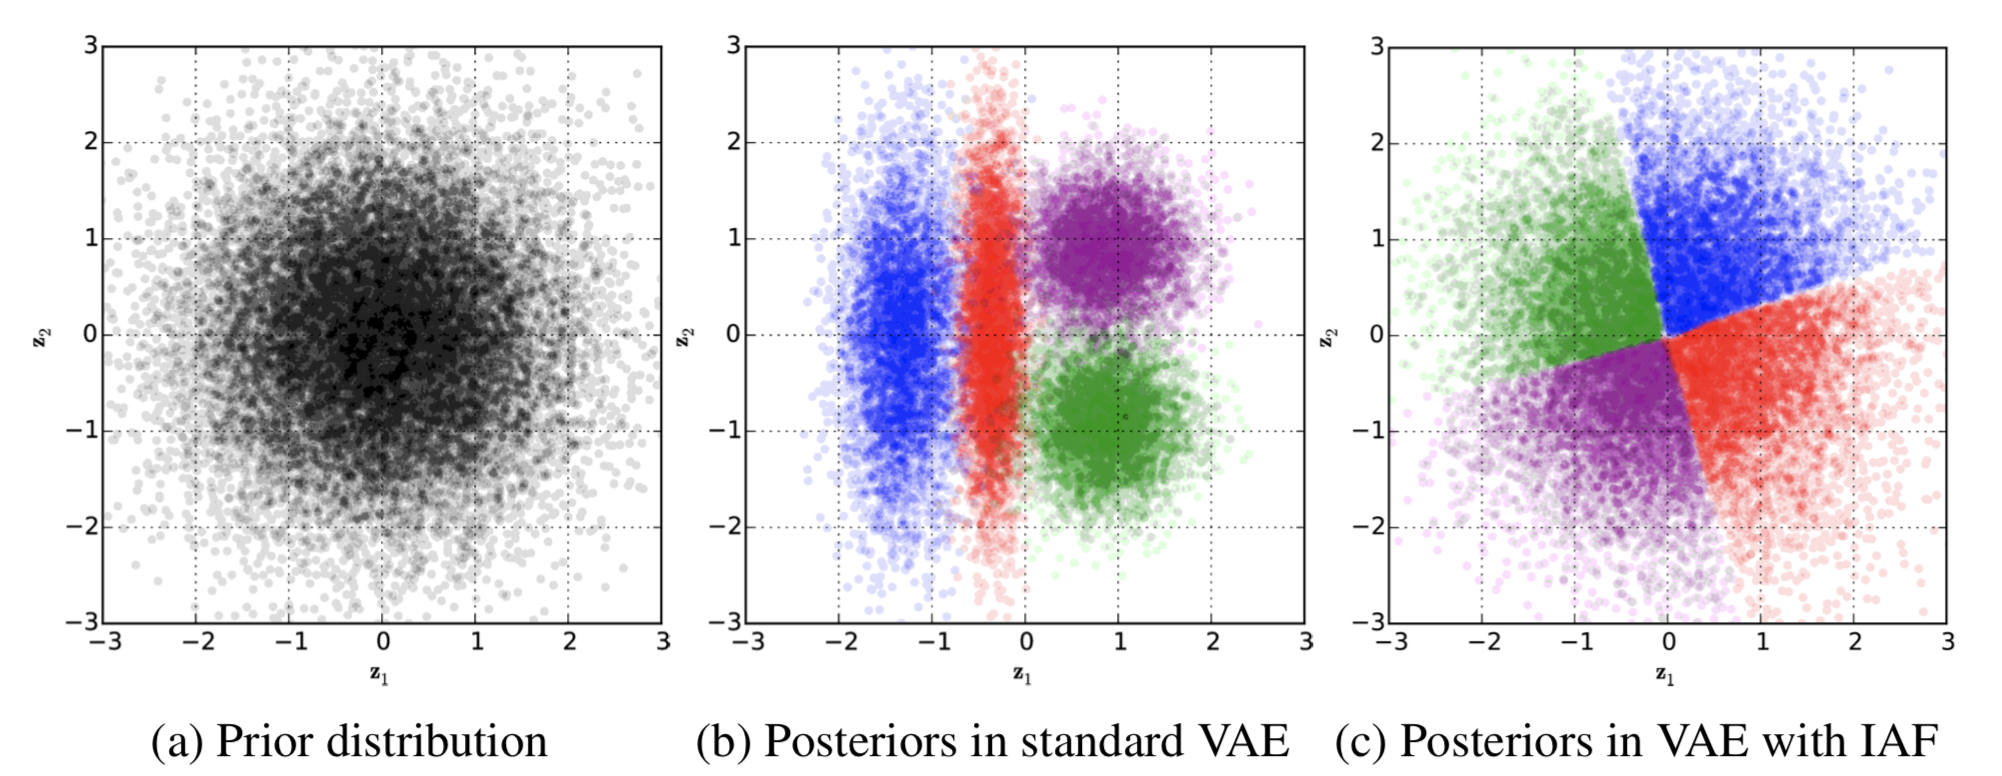
\includegraphics[width=\linewidth]{figs/iaf1.png}
	\end{figure}

	\myfootnotewithlink{https://arxiv.org/abs/1606.04934}{Kingma D. P. et al. Improving Variational Inference with Inverse Autoregressive Flow, 2016} 
\end{frame}
%=======
\begin{frame}{Flows-based VAE prior vs posterior}
	\begin{block}{Theorem}
	VAE with the flow-based prior for latent code $\bz$ is equivalent to using flow-based posterior for latent code $\bepsilon$.
	\end{block}
	\begin{block}{Proof}
	\vspace{-0.5cm}
	\begin{align*}
		\mathcal{L}(\bphi, \btheta, \blambda) &= \mathbb{E}_{q(\bz | \bx, \bphi)} \log p(\bx | \bz, \btheta) - \underbrace{KL( q(\bz | \bx, \bphi) || p(\bz | \blambda))}_{\text{flow-based prior}} \\
		& = \mathbb{E}_{q(\bz | \bx, \bphi)} \log p(\bx | \bz, \btheta) - \underbrace{KL( q(\bz | \bx, \bphi, \blambda) || p(\bz))}_{\text{flow-based posterior}}
	\end{align*}
	(Here we use Flow KL duality theorem from Lecture 4)
	\end{block}
	\begin{block}{Flows in VAE posterior}
		\vspace{-0.3cm}
		{\small
		\[
			\mathcal{L} (\bphi, \btheta, \blambda) 
			= \mathbb{E}_{q(\bz | \bx, \bphi)} \bigg[\log p(\bx, \bz^* | \btheta) -  \log q(\bz | \bx, \bphi ) +   \log \left| \det \left( \frac{\partial f(\bz, \blambda)}{\partial \bz} \right) \right| \bigg].
		\]
		}
	\end{block}
	\myfootnotewithlink{https://arxiv.org/abs/1611.02731}{Chen X. et al. Variational Lossy Autoencoder, 2016}
\end{frame}
%=======
\begin{frame}{Flows-based VAE prior vs posterior}
	\begin{itemize}
		\item IAF posterior decoder path: $p(\bx|\bz, \btheta)$, $\bz \sim p(\bz)$.
		\item AF prior decoder path: $p(\bx|\bz, \btheta)$, $\bz = g(\bepsilon, \blambda)$, $\bepsilon \sim p(\bepsilon)$. 
	\end{itemize}
	The AF prior and the IAF posterior have the same computation cost, so using the AF prior makes the model more expressive at no training time cost.

	\begin{figure}
		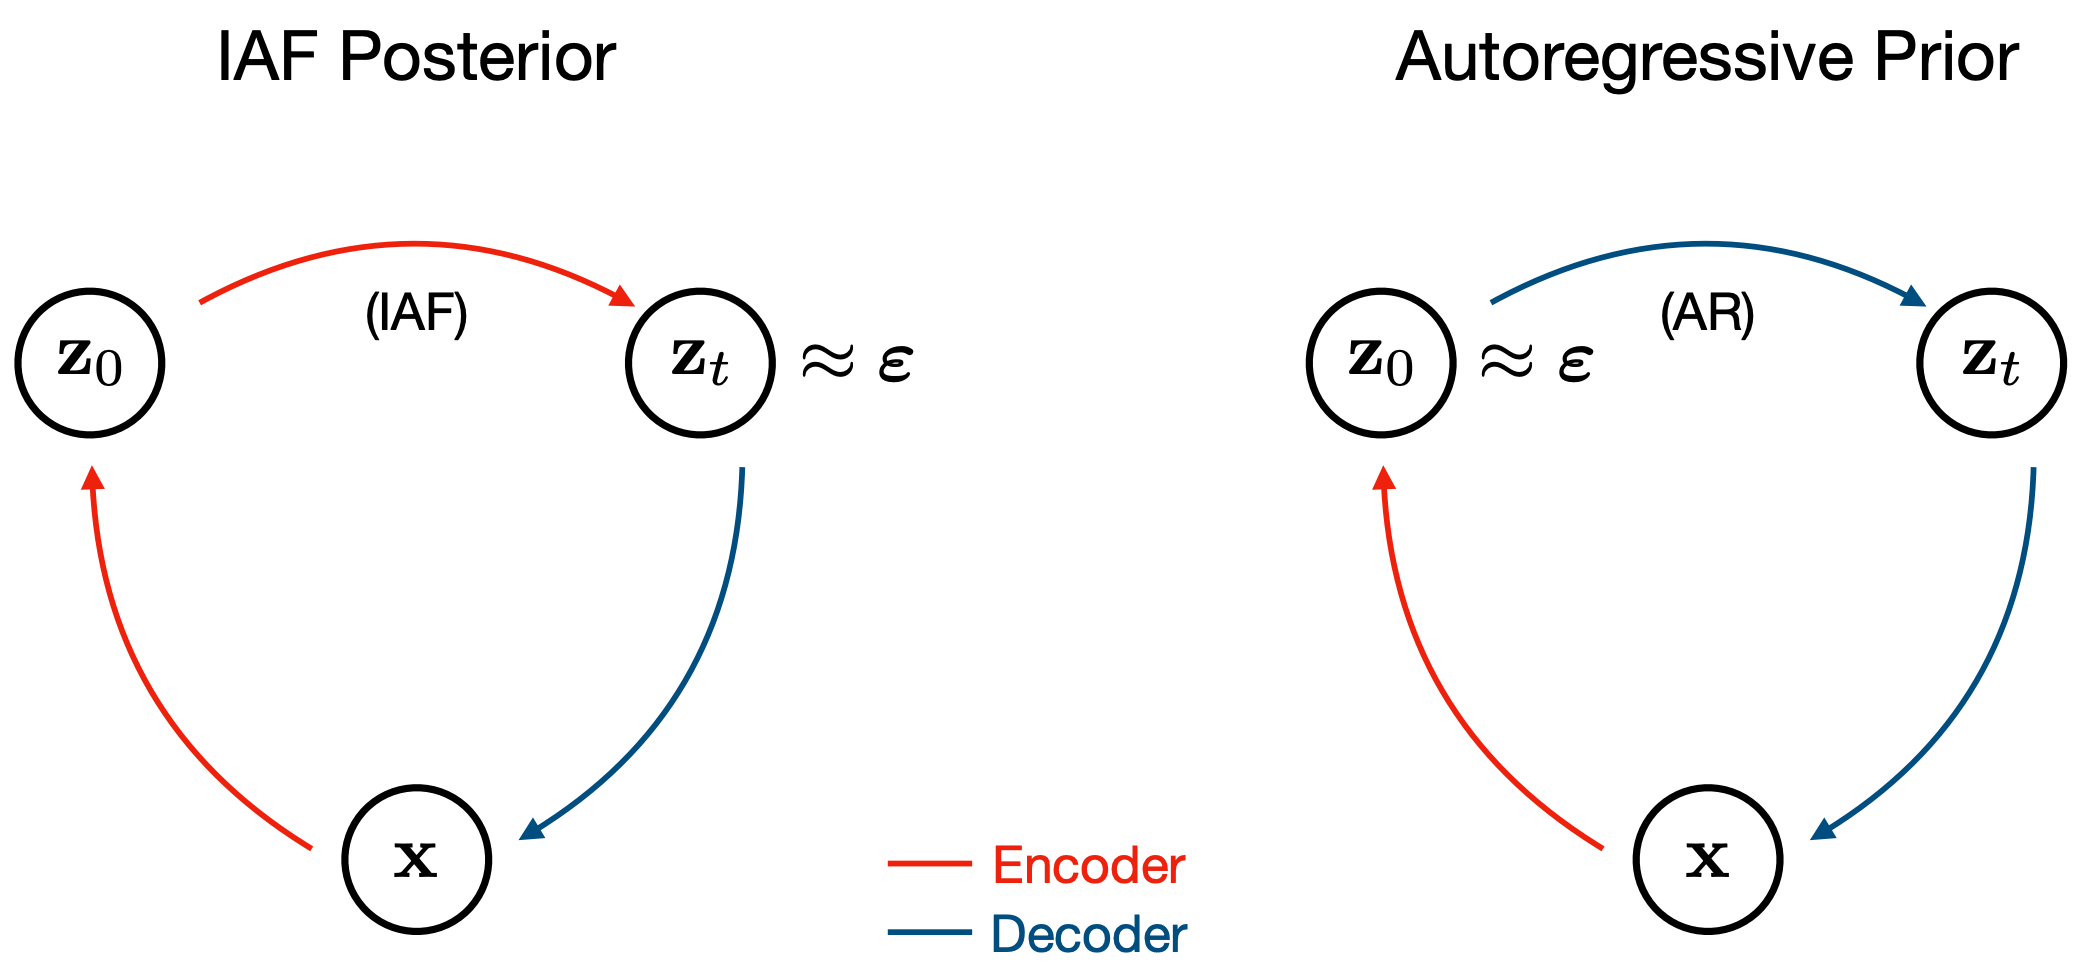
\includegraphics[width=0.9\linewidth]{figs/prior_vs_posterior}
	\end{figure}

	\myfootnotewithlink{https://courses.cs.washington.edu/courses/cse599i/20au/slides/L09_flow.pdf}{image credit: https://courses.cs.washington.edu/courses/cse599i/20au}
\end{frame}
\begin{frame}{Recap of previous lecture}
	\begin{block}{ELBO}
		\vspace{-0.3cm}
		\[
			p(\bx | \btheta) \geq \mathcal{L} (\bphi, \btheta)  = \mathbb{E}_{q(\bz | \bx, \bphi)} \log \frac{p(\bx, \bz | \btheta)}{q(\bz| \bx, \bphi)} \rightarrow \max_{\bphi, \btheta}.
		\]
		\vspace{-0.5cm}
	\end{block}
		\begin{itemize}
			\item Normal variational distribution $q(\bz | \bx, \bphi) = \mathcal{N}(\bz| \bmu_{\bphi}(\bx), \bsigma^2_{\bphi}(\bx))$ is poor (e.g. has only one mode). \\
			\item Flows models convert a simple base distribution to a compex one using an invertible transformation with simple Jacobian. 
		\end{itemize}
	\begin{block}{Flow model in latent space}
		\vspace{-0.7cm}
		\[
			\log q_K(\bz_K | \bx, \bphi_*) = \log q(\bz_0 | \bx, \bphi) - \sum_{k=1}^K \log \left| \det \left( \frac{\partial g_k(\bz_{k - 1}, \bphi_k)}{\partial \bz_{k-1}} \right) \right|.
		\]
		\vspace{-0.5cm}
	\end{block}
	Let's use $q_K(\bz_K | \bx, \bphi_*), \, \bphi_* = \{\bphi, \bphi_1, \dots, \bphi_K\}$ as a variational distribution. Here, $\bphi$~-- encoder parameters, $\{\bphi_k\}_{k=1}^K$~-- flow parameters.
	
	\myfootnotewithlink{https://arxiv.org/abs/1505.05770}{Rezende D. J., Mohamed S. Variational Inference with Normalizing Flows, 2015} 
\end{frame}
%=======
\begin{frame}{Recap of previous lecture}
	\begin{block}{Variational distribution}
		\vspace{-0.6cm}
		\[
			\log q_K(\bz_K | \bx, \bphi_*) = \log q(\bz_0 | \bx, \bphi) - \sum_{k=1}^K \log \left| \det \left( \frac{\partial g_k(\bz_{k - 1}, \bphi_k)}{\partial \bz_{k-1}} \right) \right|.
		\]
		\vspace{-0.6cm}
	\end{block}
	\begin{block}{ELBO objective}
		\vspace{-0.7cm}
		\begin{align*}
			\mathcal{L} (\bphi, \btheta) 
			&= \mathbb{E}_{q(\bz_0 | \bx, \bphi)} \bigg[\log p(\bx, \bz_K | \btheta) -  \log q(\bz_0 | \bx, \bphi ) + \\ & \quad  + \sum_{k=1}^K \log \left| \det \left( \frac{\partial g_k(\bz_{k - 1}, \bphi_k)}{\partial \bz_{k-1}} \right) \right| \bigg].
		\end{align*}
		\vspace{-0.5cm}
	\end{block}
	\begin{itemize}
		\item Obtain samples $\bz_0$ from the encoder.
		\item Apply flow model $\bz_K = g(\bz_0, \{\bphi_k\}_{k = 1}^K)$.
		\item Compute likelihood for $\bz_K$ using the decoder, base distribution for $\bz_0$ and the Jacobian.
		\item We do not need an inverse flow function if we use flows in variational inference.
	\end{itemize}
	\myfootnotewithlink{https://arxiv.org/abs/1505.05770}{Rezende D. J., Mohamed S. Variational Inference with Normalizing Flows, 2015} 
\end{frame}
%=======
\begin{frame}{Recap of previous lecture}
	Images are discrete data flow is a continuous model.
	We need to convert a discrete data distribution to a continuous one.
	
	\begin{block}{Uniform dequantization bound}
		\vspace{-0.5cm}
		\[
			\bx \sim \text{Categorical}(\bpi), \quad 
			\bu \sim U[0, 1], \quad 
			\by = \bx + \bu \sim \text{Continuous} 
		\]
		\vspace{-0.4cm}
		\[
			\log P(\bx | \btheta) \geq \int_{U[0, 1]} \log p(\bx + \bu | \btheta) d \bu.
		\]
	\end{block}
	\vspace{-0.2cm}
	\begin{block}{Variational dequantization bound}
		Introduce variational dequantization noise distribution $q(\bu | \bx)$ and treat it as an approximate posterior. 
		\vspace{-0.2cm}
		\[
			\log P(\bx | \btheta) \geq  \int q(\bu | \bx) \log \frac{p(\bx + \bu | \btheta)}{q(\bu | \bx)} d \bu = \mathcal{L}(q, \btheta).
		\]
	\end{block}
	\myfootnotewithlink{https://arxiv.org/abs/1902.00275}{Ho J. et al. Flow++: Improving Flow-Based Generative Models with Variational Dequantization and Architecture Design, 2019}
\end{frame}
%=======
\begin{frame}{Recap of previous lecture}
	
	\begin{minipage}[t]{0.5\columnwidth}
		\begin{figure}
			\centering
			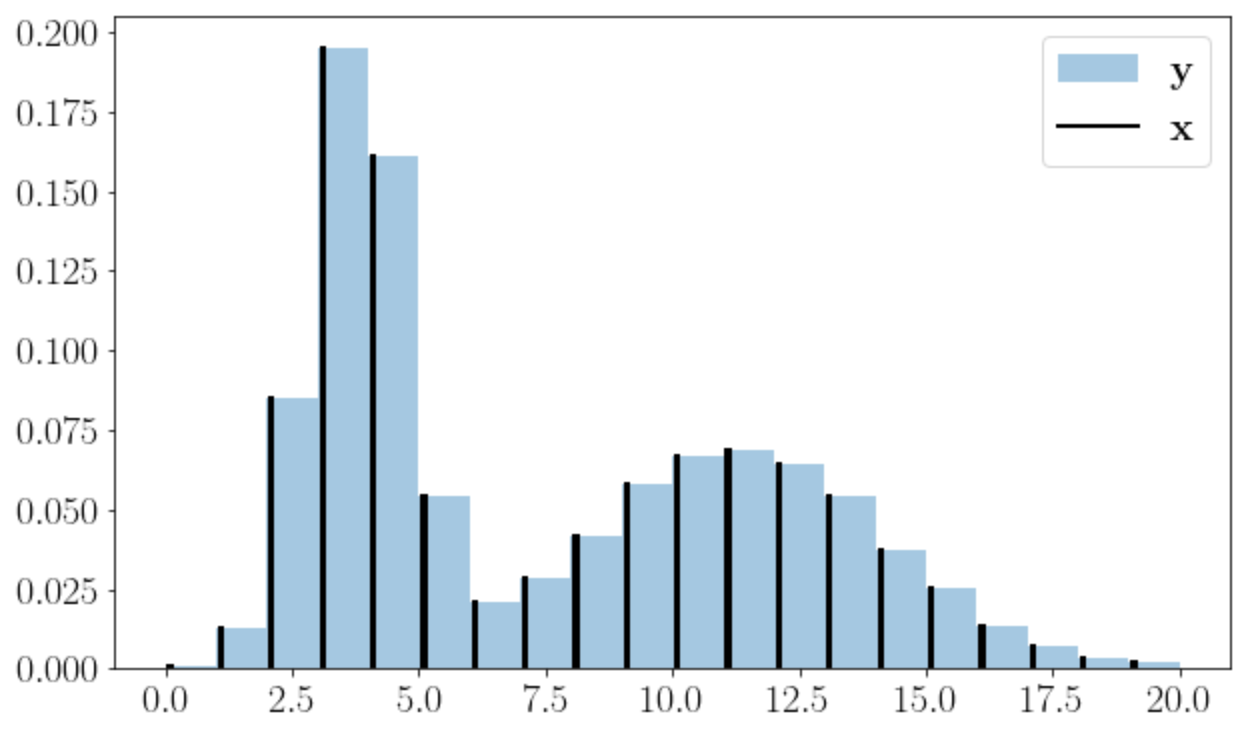
\includegraphics[width=1.0\linewidth]{figs/uniform_dequantization.png}
		\end{figure}
	\end{minipage}%
	\begin{minipage}[t]{0.5\columnwidth}
		\begin{figure}
			\centering
			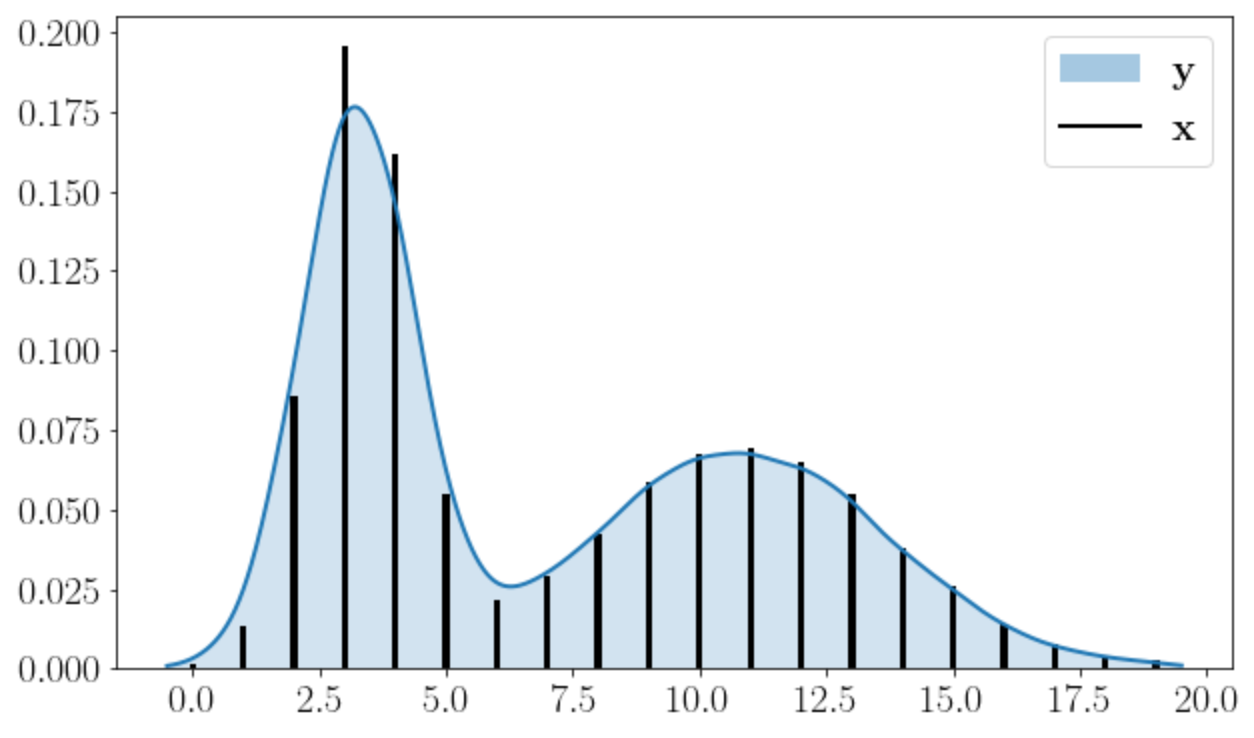
\includegraphics[width=1.0\linewidth]{figs/variational_dequantization.png}
		\end{figure}
	\end{minipage}
	\begin{block}{Flow model for dequantization}
	\vspace{-0.3cm}
	\[
	q(\bu | \bx) = p(h^{-1}(\bu, \bphi)) \cdot \left| \det \frac{\partial h^{-1}(\bu, \bphi)}{\partial \bu}\right|.
	\]
	\vspace{-0.3cm}
	\end{block}
	\begin{block}{Variational dequantization bound}
		\[
		\mathcal{L}(q, \btheta) = \int q(\bu | \bx) \log \frac{p(\bx + \bu | \btheta)}{q(\bu | \bx)} d \bu.
		\]
	\end{block}
	\myfootnotewithlink{https://arxiv.org/abs/1902.00275}{Ho J. et al. Flow++: Improving Flow-Based Generative Models with Variational Dequantization and Architecture Design, 2019}
\end{frame}
%=======
\begin{frame}{Recap of previous lecture}
	\vspace{-0.3cm}
	\[
	\frac{1}{n} \sum_{i=1}^n \mathcal{L}_i(q, \btheta) = \frac{1}{n} \sum_{i=1}^n \left[ \mathbb{E}_{q(\bz | \bx_i)} \log p(\bx_i | \bz, \btheta) - KL(q(\bz | \bx_i) || p(\bz)) \right].
	\]
	\vspace{-0.3cm}
	\begin{block}{Theorem}
		\[
		\frac{1}{n} \sum_{i=1}^n KL(q(\bz | \bx_i) || p(\bz)) = KL(q(\bz) || p(\bz)) + \bbI_{q} [\bx, \bz],
		\]
		\begin{itemize}
			\item $q(\bz) = \frac{1}{n} \sum_{i=1}^n q(\bz | \bx_i)$ -- \textbf{aggregated} posterior distribution.
			\item $\bbI_{q} [\bx, \bz]$ -- mutual information between $\bx$ and $\bz$ under empirical data distribution and distribution $q(\bz | \bx)$.
			\item First term pushes $q(\bz)$ towards the prior $p(\bz)$.
			\item Second term reduces the amount of	information about $\bx$ stored in $\bz$. 
		\end{itemize}
	\end{block}
	\myfootnotewithlink{http://approximateinference.org/accepted/HoffmanJohnson2016.pdf}{Hoffman M. D., Johnson M. J. ELBO surgery: yet another way to carve up the variational evidence lower bound, 2016}
\end{frame}
%=======
\begin{frame}{Dequantization}
	\begin{itemize}
		\item Images are discrete data, pixels lie in the [0, 255] integer domain (the model is $P(\bx | \btheta) = \text{Categorical}(\bpi(\btheta))$).
		\item Flow is a continuous model (it works with continuous data $\bx$).
	\end{itemize}
	By fitting a continuous density model to discrete data, one can produce a degenerate solution with all probability mass on discrete values. \\
	How to convert a discrete data distribution to a continuous one?
	
	\begin{minipage}[t]{0.5\columnwidth}
		\begin{block}{Uniform dequantization}
		\vspace{-0.5cm}
			\begin{align*}
				\bx &\sim \text{Categorical}(\bpi) \\
				 \bu &\sim U[0, 1]
			\end{align*}
			\[
			\by = \bx + \bu \sim \text{Continuous} 
			\]
		\end{block}
	\end{minipage}%
	\begin{minipage}[t]{0.5\columnwidth}
		\begin{figure}
			\centering
			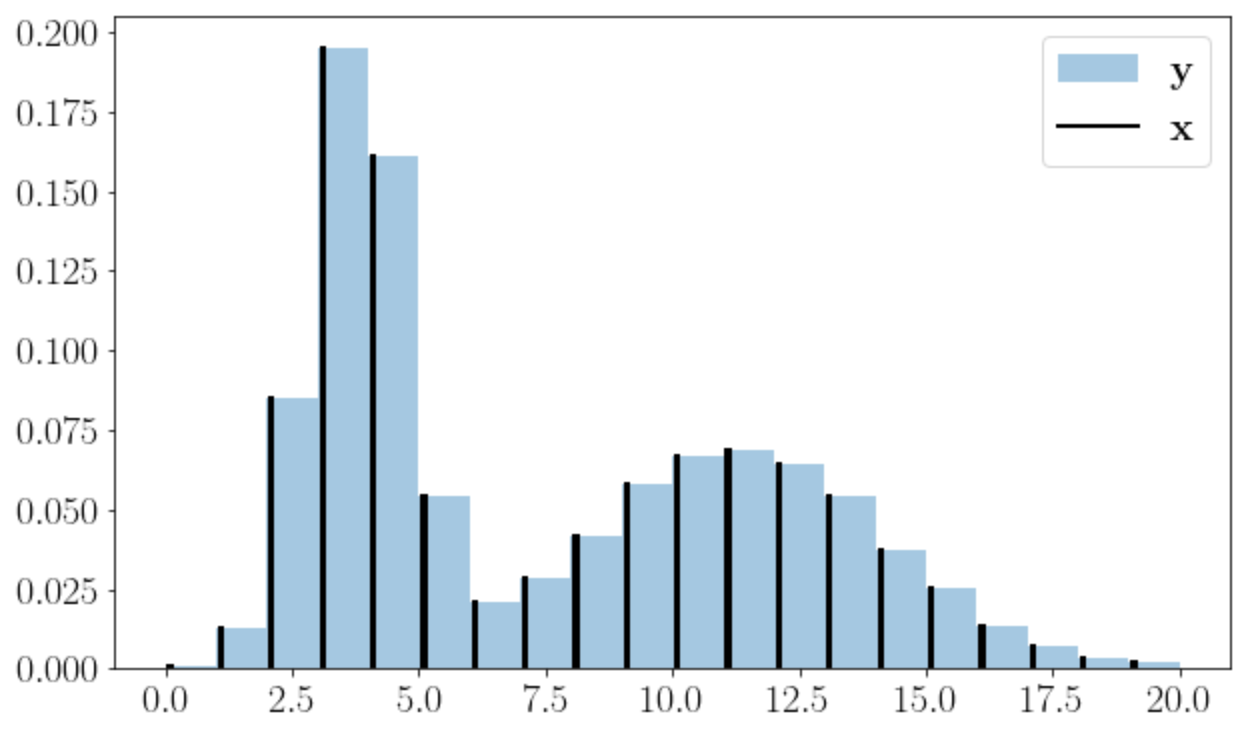
\includegraphics[width=1.0\linewidth]{figs/uniform_dequantization.png}
		\end{figure}
	\end{minipage}
	\myfootnotewithlink{https://arxiv.org/abs/1511.01844}{Theis L., Oord A., Bethge M. A note on the evaluation of generative models. 2015}
\end{frame}
%=======
\begin{frame}{Uniform dequantization}
	\begin{block}{Statement}
		Fitting continuous model $p(\by | \btheta)$ on uniformly dequantized data $\by = \bx + \bu, \, \bu \sim U[0, 1]$ is equivalent to maximization of a lower bound on log-likelihood for a discrete model:
		\[
		P(\bx | \btheta) = \int_{U[0, 1]} p(\bx + \bu | \btheta) d \bu
		\]
		\vspace{-0.2cm} \\
		Thus, the maximisation of continuous model log-likelihood on $\by$ can't lead to the a collapse onto the discrete data (the objective is bounded above by the discrete model log-likelihood).
	\end{block}
	\begin{block}{Proof}
		\vspace{-1cm}
		\begin{multline*}
			 \log P(\bx | \btheta) = \log \int_{U[0, 1]} p(\bx + \bu | \btheta) d \bu \geq \\ \geq \int_{U[0, 1]} \log p(\bx + \bu | \btheta) d \bu = \log p(\by | \btheta).
		\end{multline*}
	\end{block}
\end{frame}
%=======
\begin{frame}{Dequantization}
	\begin{itemize}
		\item Images are discrete data, pixels lie in the \{0, 255\} integer domain (the model is $P(\bx | \btheta) = \text{Categorical}(\bpi(\btheta))$).
		\item Flow is a continuous model (it works with continuous data $\bx$).
	\end{itemize}
	By fitting a continuous density model to discrete data, one can produce a degenerate solution with all probability mass on discrete values. \\
	How to convert a discrete data distribution to a continuous one?
	
	\begin{minipage}[t]{0.5\columnwidth}
		\begin{block}{Uniform dequantization}
		\vspace{-0.5cm}
			\begin{align*}
				\bx &\sim \text{Categorical}(\bpi) \\
				 \bu &\sim U[0, 1]
			\end{align*}
			\[
			\by = \bx + \bu \sim \text{Continuous} 
			\]
		\end{block}
	\end{minipage}%
	\begin{minipage}[t]{0.5\columnwidth}
		\begin{figure}
			\centering
			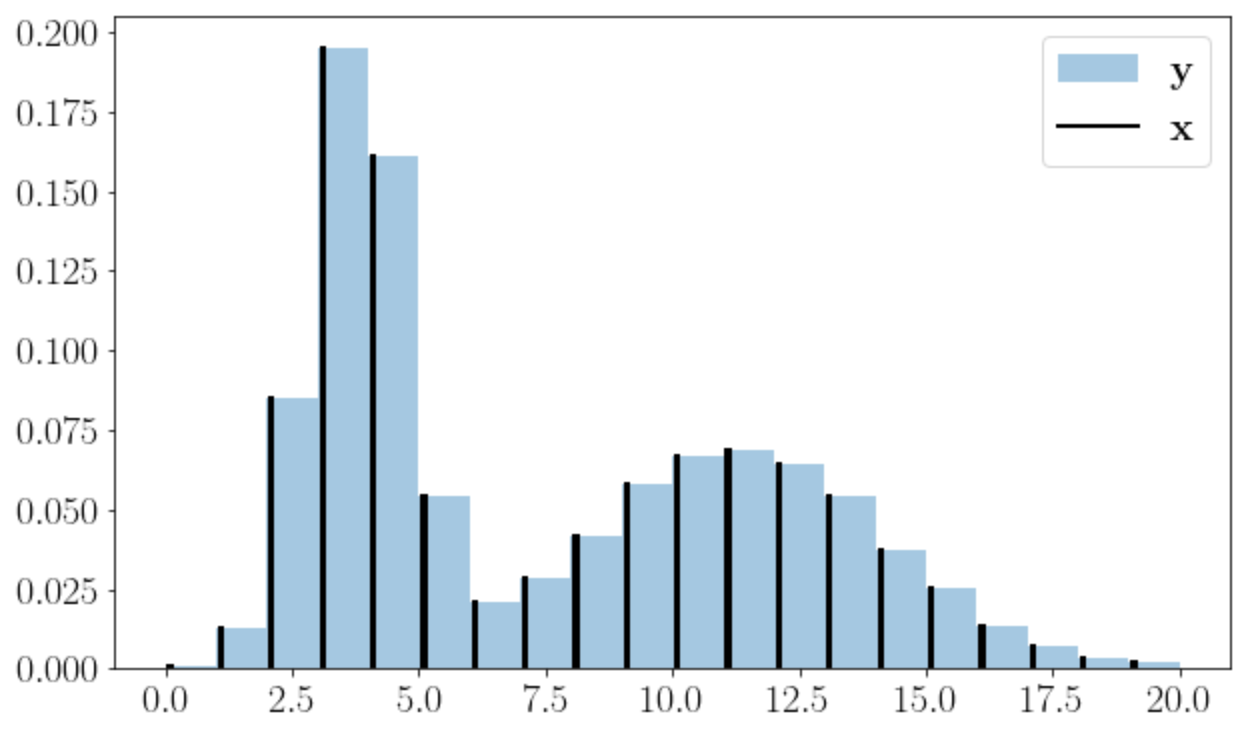
\includegraphics[width=1.0\linewidth]{figs/uniform_dequantization.png}
		\end{figure}
	\end{minipage}
	\myfootnotewithlink{https://arxiv.org/abs/1511.01844}{Theis L., Oord A., Bethge M. A note on the evaluation of generative models. 2015}
\end{frame}
%=======
\begin{frame}{Uniform dequantization}
	\begin{block}{Statement}
		Fitting continuous model $p(\by | \btheta)$ on uniformly dequantized data $\by = \bx + \bu, \, \bu \sim U[0, 1]$ is equivalent to maximization of a lower bound on log-likelihood for a discrete model:
		\vspace{-0.2cm}
		\[
		P(\bx | \btheta) = \int_{U[0, 1]} p(\bx + \bu | \btheta) d \bu
		\]
		\vspace{-0.5cm} 
	\end{block}
	\begin{block}{Proof}
		\vspace{-0.8cm}
		\begin{multline*}
			\bbE_{\pi} \log p(\by | \btheta) = \int \pi(\by) \log p(\by | \btheta) d \by = \\ 
			= \sum \pi(\bx) \int_{U[0,1]} \log p(\bx + \bu | \btheta) d \bu \leq \\
			 \leq \sum \pi(\bx) \log \int_{U[0,1]}  p(\bx + \bu | \btheta) d \bu = \\
			 = \sum \pi(\bx) \log P(\bx | \btheta) = \bbE_{\pi} \log P(\bx | \btheta).
		\end{multline*}
	\end{block}
	\myfootnotewithlink{https://arxiv.org/abs/1511.01844}{Theis L., Oord A., Bethge M. A note on the evaluation of generative models. 2015}
\end{frame}
%=======
\begin{frame}{Variational dequantization}
	\begin{minipage}[t]{0.5\columnwidth}
			\begin{figure}
				\centering
				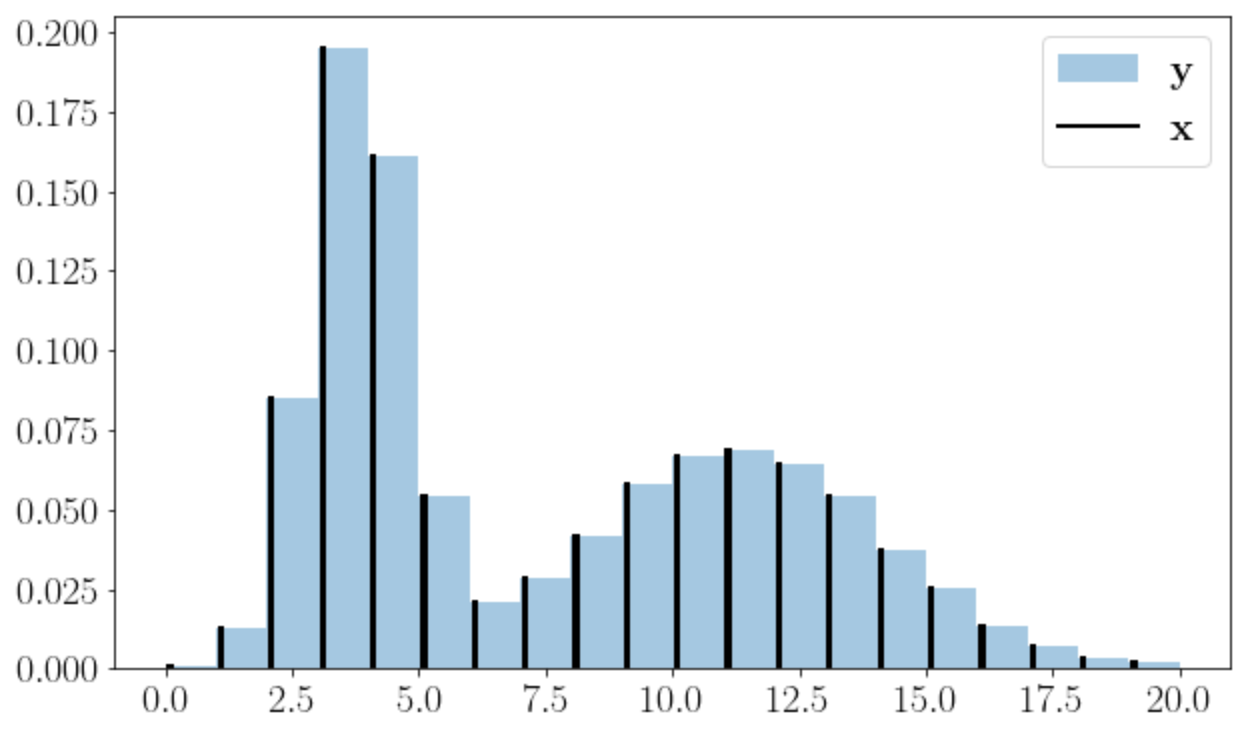
\includegraphics[width=1.0\linewidth]{figs/uniform_dequantization.png}
			\end{figure}
	\end{minipage}%
	\begin{minipage}[t]{0.5\columnwidth}
		\begin{figure}
			\centering
			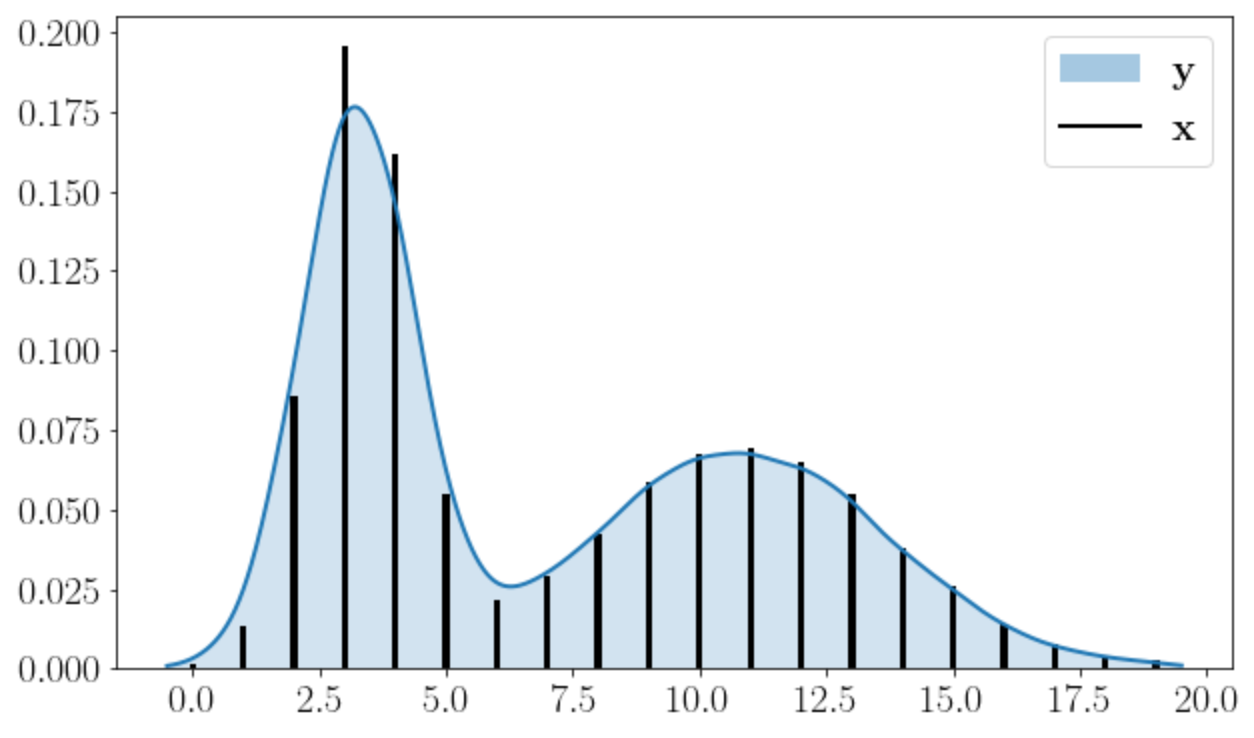
\includegraphics[width=1.0\linewidth]{figs/variational_dequantization.png}
		\end{figure}
	\end{minipage}
	\begin{itemize}
		\item $p(\by | \btheta)$ assign unifrom density to unit hypercubes $\bx + U[0, 1]$ (left fig).
		\item Neural network density models are smooth function approximators (right fig).
		\item Smooth dequantization is more natural.
	\end{itemize}
	How to perform the smooth dequantization? \\
\end{frame}
%=======
\begin{frame}{Flow++}
	\begin{block}{Variational dequantization}
		Introduce variational dequantization noise distribution $q(\bu | \bx)$ and treat it as an approximate posterior. 
	\end{block}
	\begin{block}{Variational lower bound}
		\vspace{-0.7cm}
		\begin{multline*}
		 \log P(\bx | \btheta) = \left[ \log \int q(\bu | \bx) \frac{p(\bx + \bu | \btheta)}{q(\bu | \bx)} d \bu \right] \geq \\ 
			\geq  \int q(\bu | \bx) \log \frac{p(\bx + \bu | \btheta)}{q(\bu | \bx)} d \bu = \mathcal{L}(q, \btheta).
		\end{multline*}
	\end{block}
	\vspace{-0.5cm}
	\begin{block}{Uniform dequantization bound}
		\vspace{-0.4cm}
		\[
		 \log P(\bx | \btheta) = \log \int_{U[0, 1]} p(\bx + \bu | \btheta) d \bu \geq \int_{U[0, 1]} \log p(\bx + \bu | \btheta) d \bu.
		\]
	\end{block}
	\myfootnotewithlink{https://arxiv.org/abs/1902.00275}{Ho J. et al. Flow++: Improving Flow-Based Generative Models with Variational Dequantization and Architecture Design, 2019}
\end{frame}
%=======
\begin{frame}{Flow++}
	\begin{block}{Variational lower bound}
		\[
		\mathcal{L}(q, \btheta) = \int q(\bu | \bx) \log \frac{p(\bx + \bu | \btheta)}{q(\bu | \bx)} d \bu.
		\]
	\end{block}
	Let $\bu = h(\bepsilon, \bphi)$ is a flow model with base distribution $\bepsilon \sim p(\bepsilon) = \mathcal{N}(0, \mathbf{I})$:
	\vspace{-0.3cm}
	\[
		q(\bu | \bx) = p(h^{-1}(\bu, \bphi)) \cdot \left| \det \frac{\partial h^{-1}(\bu, \bphi)}{\partial \bu}\right|.
	\]
	\vspace{-0.3cm}
	Then
	\[
		\log P(\bx | \btheta) \geq \cL(\bphi, \btheta) = \int p(\bepsilon) \log \left( \frac{p(\bx + h(\bepsilon, \bphi) | \btheta)}{p(\bepsilon) \cdot \left| \det \frac{\partial h(\bepsilon, \bphi)}{\partial \bepsilon}\right|^{-1}} \right) d\bepsilon.
	\]
	\myfootnotewithlink{https://arxiv.org/abs/1902.00275}{Ho J. et al. Flow++: Improving Flow-Based Generative Models with Variational Dequantization and Architecture Design, 2019}
\end{frame}
%=======
\begin{frame}{Flow++}
	\begin{block}{Variational lower}
	\vspace{-0.3cm}
	\[
		\log P(\bx | \btheta) \geq \int p(\bepsilon)\log \left( \frac{p(\bx + h(\bepsilon, \bphi))}{p(\bepsilon) \cdot \left| \det \frac{\partial h(\bepsilon, \bphi)}{\partial \bepsilon}\right|^{-1}} \right) d\bepsilon.
	\]
	\end{block}
	\begin{itemize}
	\item If $p(\bx + \bu | \btheta)$ is also a flow model, it is straightforward to calculate stochastic gradient of this ELBO.
	
	\item Uniform dequantization is a special case of variational dequantization ($q(\bu | \bx) = U[0, 1]$).
	The gap between $\log P(\bx | \btheta)$ and the derived ELBO is 
	$ KL(q(\bu | \bx) || p(\bu | \bx))$.
	\item In the case of uniform dequantization the model unnaturally places uniform density over each hypercube $\bx + U[0, 1]$ due to inexpressive distribution $q$.
	\end{itemize}
	\myfootnotewithlink{https://arxiv.org/abs/1902.00275}{Ho J. et al. Flow++: Improving Flow-Based Generative Models with Variational Dequantization and Architecture Design, 2019}
\end{frame}
%=======
\begin{frame}{Flow++}
	\begin{figure}
		\centering
		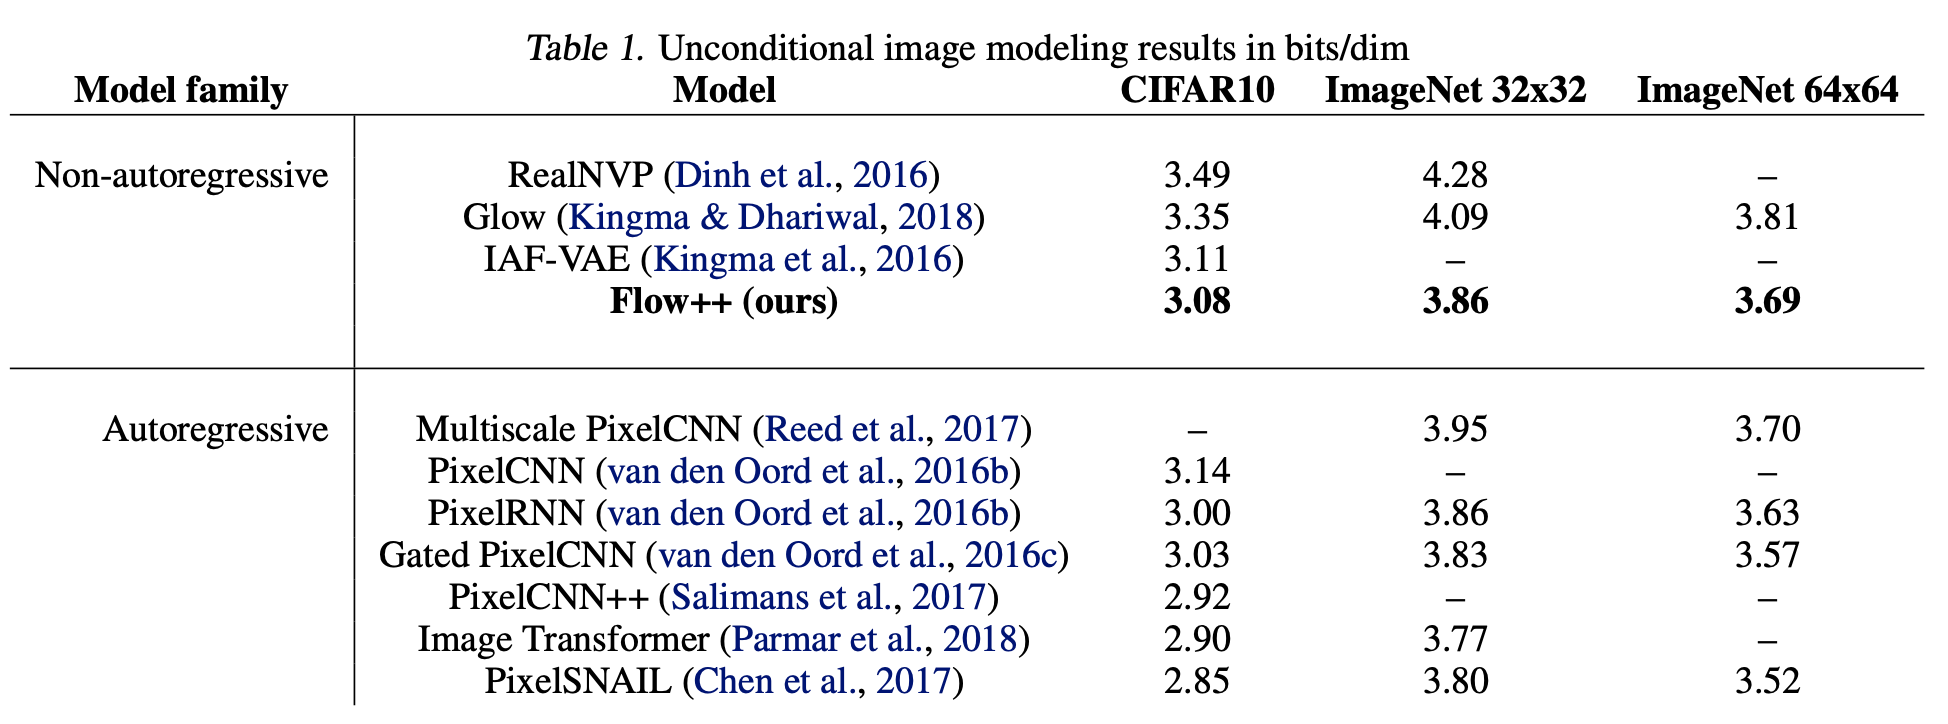
\includegraphics[width=0.7\linewidth]{figs/flow++1.png}
	\end{figure}
	\vspace{-0.1cm}
	\begin{figure}
		\centering
		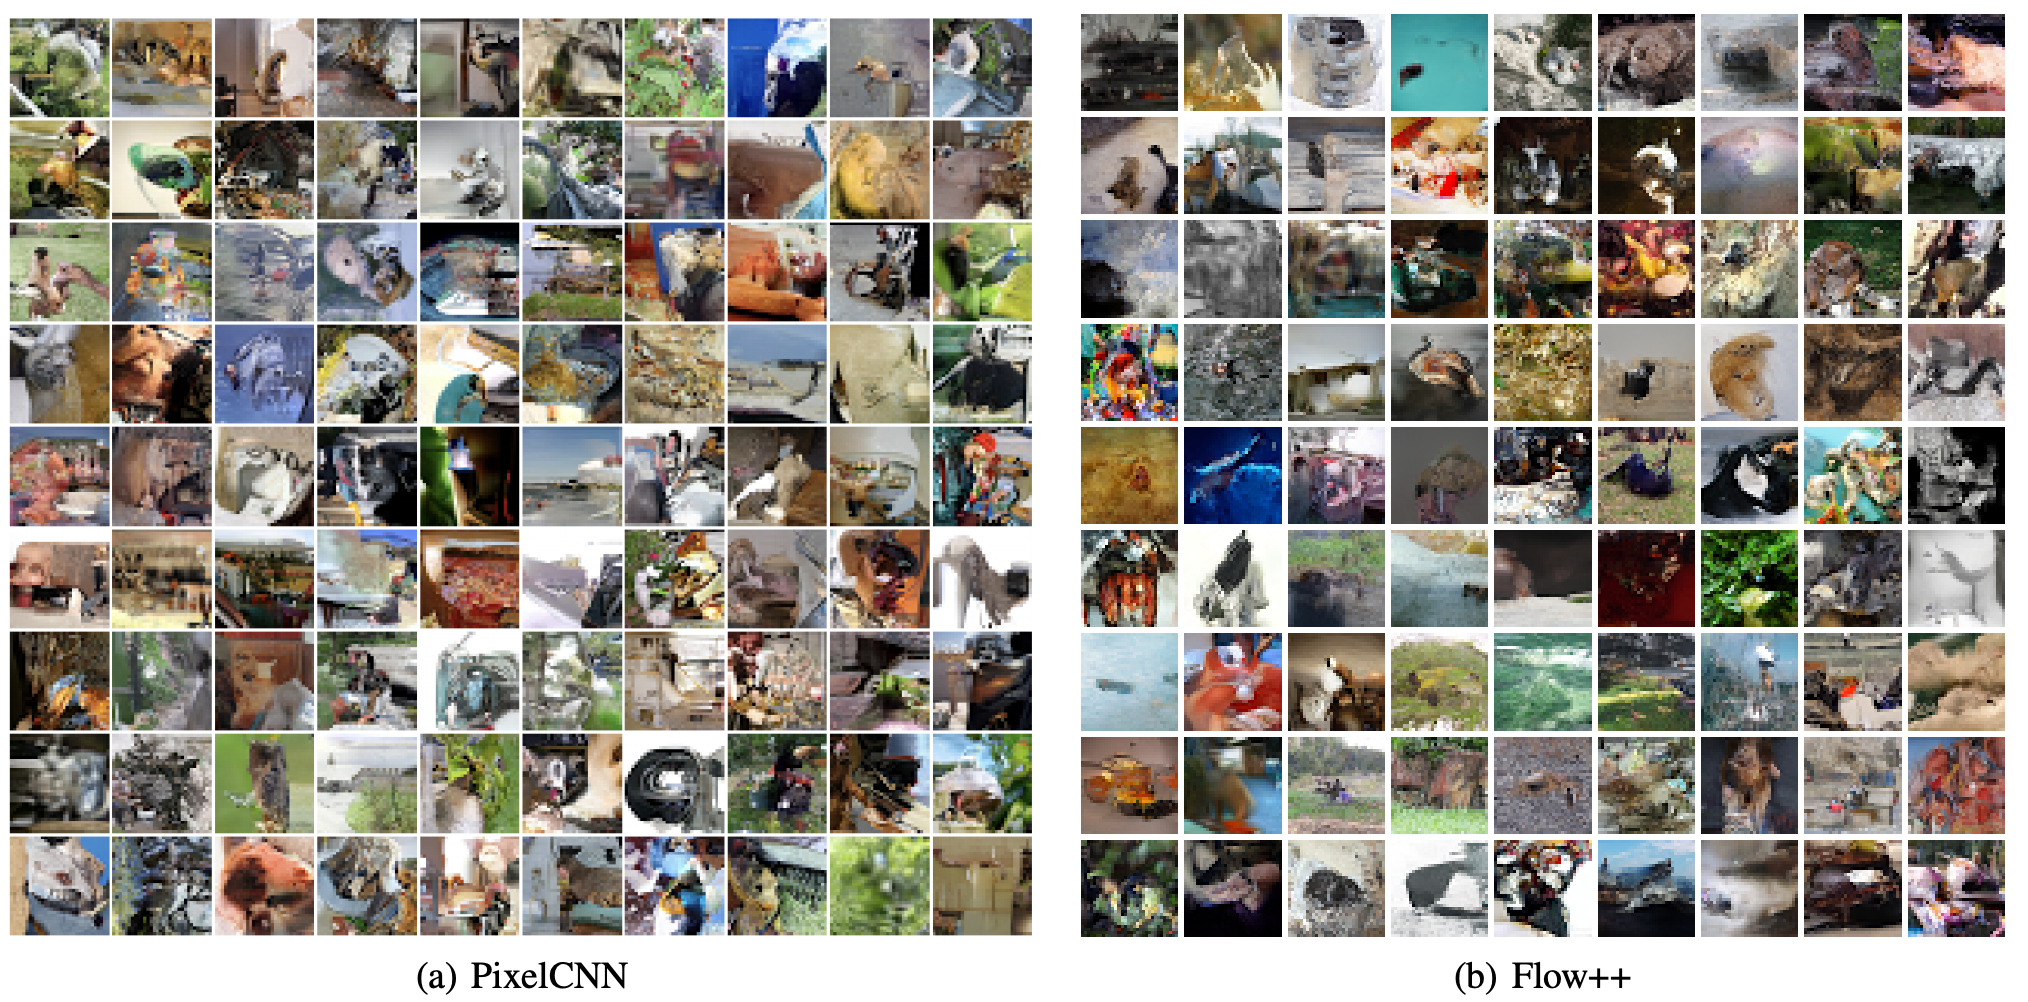
\includegraphics[width=0.8\linewidth]{figs/flow++2.png}
	\end{figure}
	\myfootnotewithlink{https://arxiv.org/abs/1902.00275}{Ho J. et al. Flow++: Improving Flow-Based Generative Models with Variational Dequantization and Architecture Design, 2019}
\end{frame}
%=======
\begin{frame}{VAE limitations}
\begin{itemize}
	\item Poor variational posterior distribution (encoder)
	\[
	q(\bz | \bx, \bphi) = \mathcal{N}(\bz| \bmu_{\bphi}(\bx), \bsigma^2_{\bphi}(\bx)).
	\]
	\item Poor prior distribution
	\[
	p(\bz) = \mathcal{N}(0, \mathbf{I}).
	\]
	\item Poor probabilistic model (decoder)
	\[
	p(\bx | \bz, \btheta) = \mathcal{N}(\bx| \bmu_{\btheta}(\bz), \bsigma^2_{\btheta}(\bz)).
	\]
	\item Loose lower bound
	\[
	\log p(\bx | \btheta) - \mathcal{L}(q, \btheta) = (?).
	\]
\end{itemize}
\end{frame}
%=======
\begin{frame}{Disentangled representations}
	\begin{block}{Unsupervised representation learning}
	    Learning an interpretable factorised representation of the independent data generative factors of the world without supervision. 
	\end{block}
	\begin{block}{Disentanglement informal definition}
	A disentangled representation can be defined as one where single latent units are sensitive to changes in single generative factors, while being relatively invariant to changes in other factors. 
	\end{block}
	\begin{block}{Example}
	Model trained on a dataset of 3D objects might learn independent latent units sensitive to single independent data generative factors, such as object identity, position, scale, lighting or colour. 
	\end{block}
	\myfootnotewithlink{https://openreview.net/references/pdf?id=Sy2fzU9gl}{Higgins I. et al. beta-VAE: Learning Basic Visual Concepts with a Constrained Variational Framework, 2017}
\end{frame}
%=======
\begin{frame}{Disentanglement learning}
	\begin{block}{Generative process}
	\begin{itemize}
	    \item $\pi(\bx | \bv, \bw) = \text{Sim}(\bv, \bw)$~-- true world simulator;
	    \item $\bv$~-- conditionally independent factors: $\pi(\bv | \bx) = \prod_{j=1}^d \pi(v_j | \bx)$;
	    \item $\bw$~-- conditionally dependent factors. 
	\end{itemize}
	\end{block}
	\begin{block}{Goal}
	Construct an unsupervised deep generative model
	\[
	    p(\bx | \bz, \btheta) \approx \pi(\bx | \bv, \bw).
	\]
	\vspace{-0.5cm}
	\begin{itemize}
	    \item Ensure that the inferred latent factors $q(\bz|\bx)$ capture the factors $\bv$ in a disentangled manner. 
	    \item The conditionally dependent factors $\bw$ can remain entangled in a separate subset of $\bz$ that is not used for representing $\bv$. 
	\end{itemize}
	\end{block}
	\myfootnotewithlink{https://openreview.net/references/pdf?id=Sy2fzU9gl}{Higgins I. et al. beta-VAE: Learning Basic Visual Concepts with a Constrained Variational Framework, 2017}
\end{frame}
%=======
\begin{frame}{$\beta$-VAE}
	\begin{block}{ELBO objective}
	\vspace{-0.2cm}
	\[
	    \mathcal{L}(q, \btheta, \beta) = \mathbb{E}_{q(\bz | \bx)} \log p(\bx | \bz, \btheta) - \beta \cdot KL (q(\bz | \bx) || p(\bz)).
	\]
	\vspace{-0.5cm}
	\end{block}
	What do we get at $\beta = 1$? \\
	\begin{block}{Constrained optimization}
		\vspace{-0.5cm}
		\[
			\max_{q, \btheta} \mathbb{E}_{q(\bz | \bx)} \log p(\bx | \bz, \btheta), \quad \text{subject to } KL (q(\bz | \bx) || p(\bz)) < \epsilon.
		\]
		\vspace{-0.5cm}
	\end{block}
	\begin{block}{Hypothesis}
	We are able to learn disentangled representations of the independent factors $\bv$ by setting a stronger constraint with $\beta > 1$.
	\end{block}
	\textbf{Note:} It leads to poorer reconstructions and a loss of high frequency details. 
	\myfootnotewithlink{https://openreview.net/references/pdf?id=Sy2fzU9gl}{Higgins I. et al. beta-VAE: Learning Basic Visual Concepts with a Constrained Variational Framework, 2017}
\end{frame}
%=======
\begin{frame}{$\beta$-VAE}
	\begin{figure}
	    \centering
	    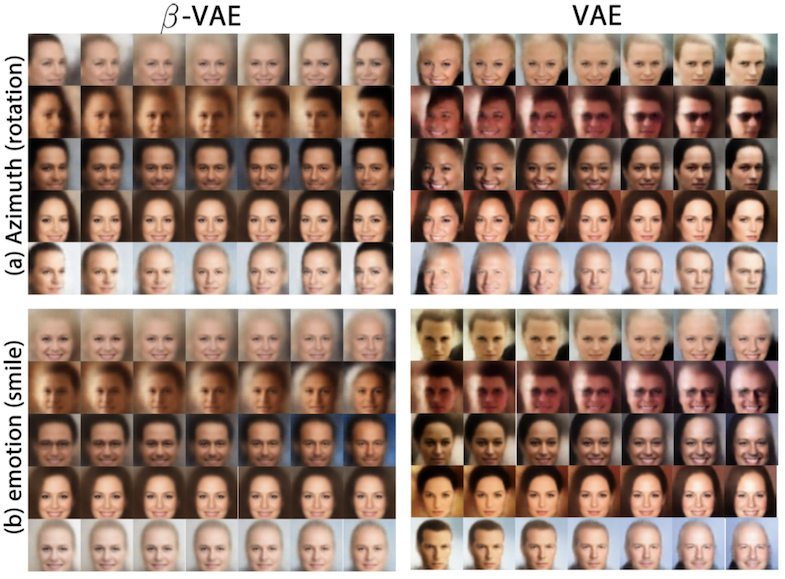
\includegraphics[width=0.95\linewidth]{figs/betaVAE_1.png}
	\end{figure}

	\myfootnotewithlink{https://openreview.net/references/pdf?id=Sy2fzU9gl}{Higgins I. et al. beta-VAE: Learning Basic Visual Concepts with a Constrained Variational Framework, 2017}
\end{frame}
%=======
\begin{frame}{$\beta$-VAE}
	\begin{figure}
	    \centering
	    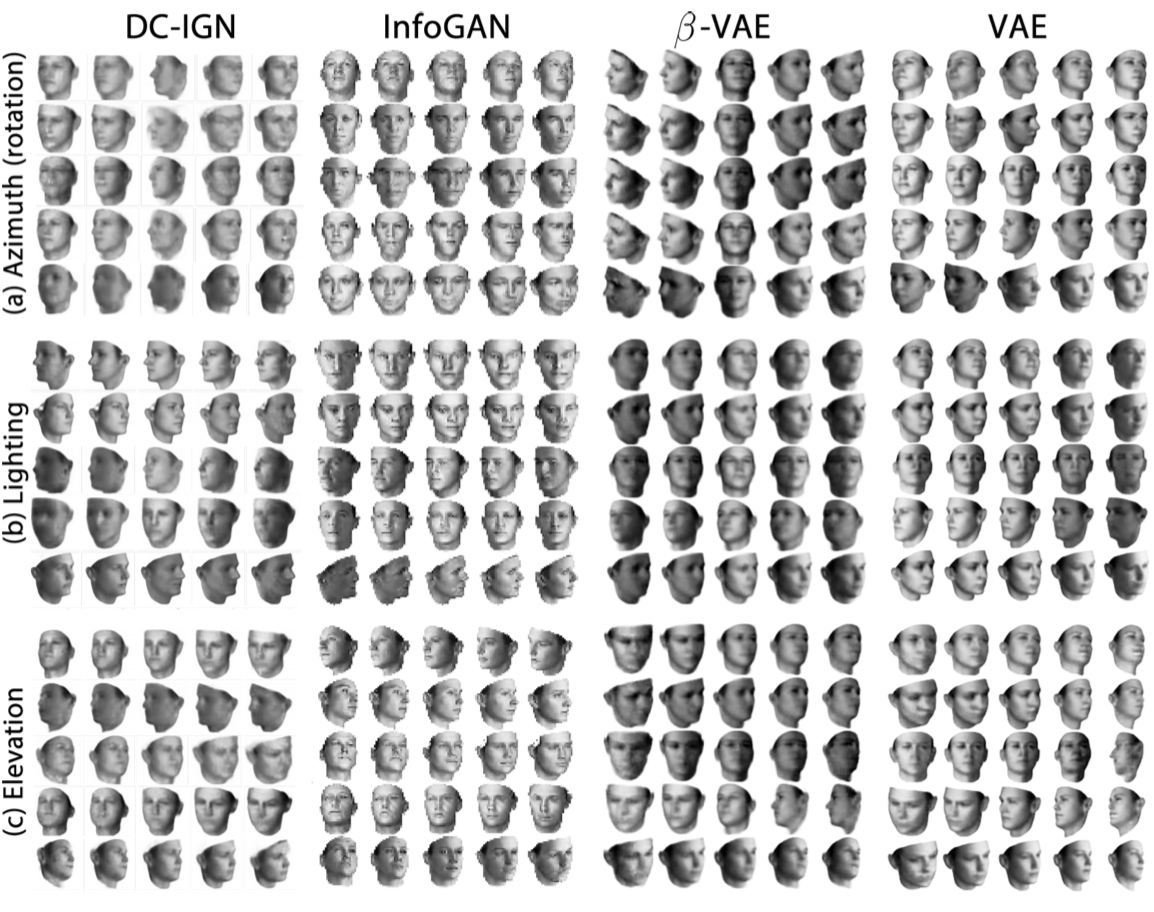
\includegraphics[width=0.9\linewidth]{figs/betaVAE_3.png}
	\end{figure}

	\myfootnotewithlink{https://openreview.net/references/pdf?id=Sy2fzU9gl}{Higgins I. et al. beta-VAE: Learning Basic Visual Concepts with a Constrained Variational Framework, 2017}
\end{frame}
%=======
\begin{frame}{$\beta$-VAE}
		\begin{figure}[h]
			\centering
			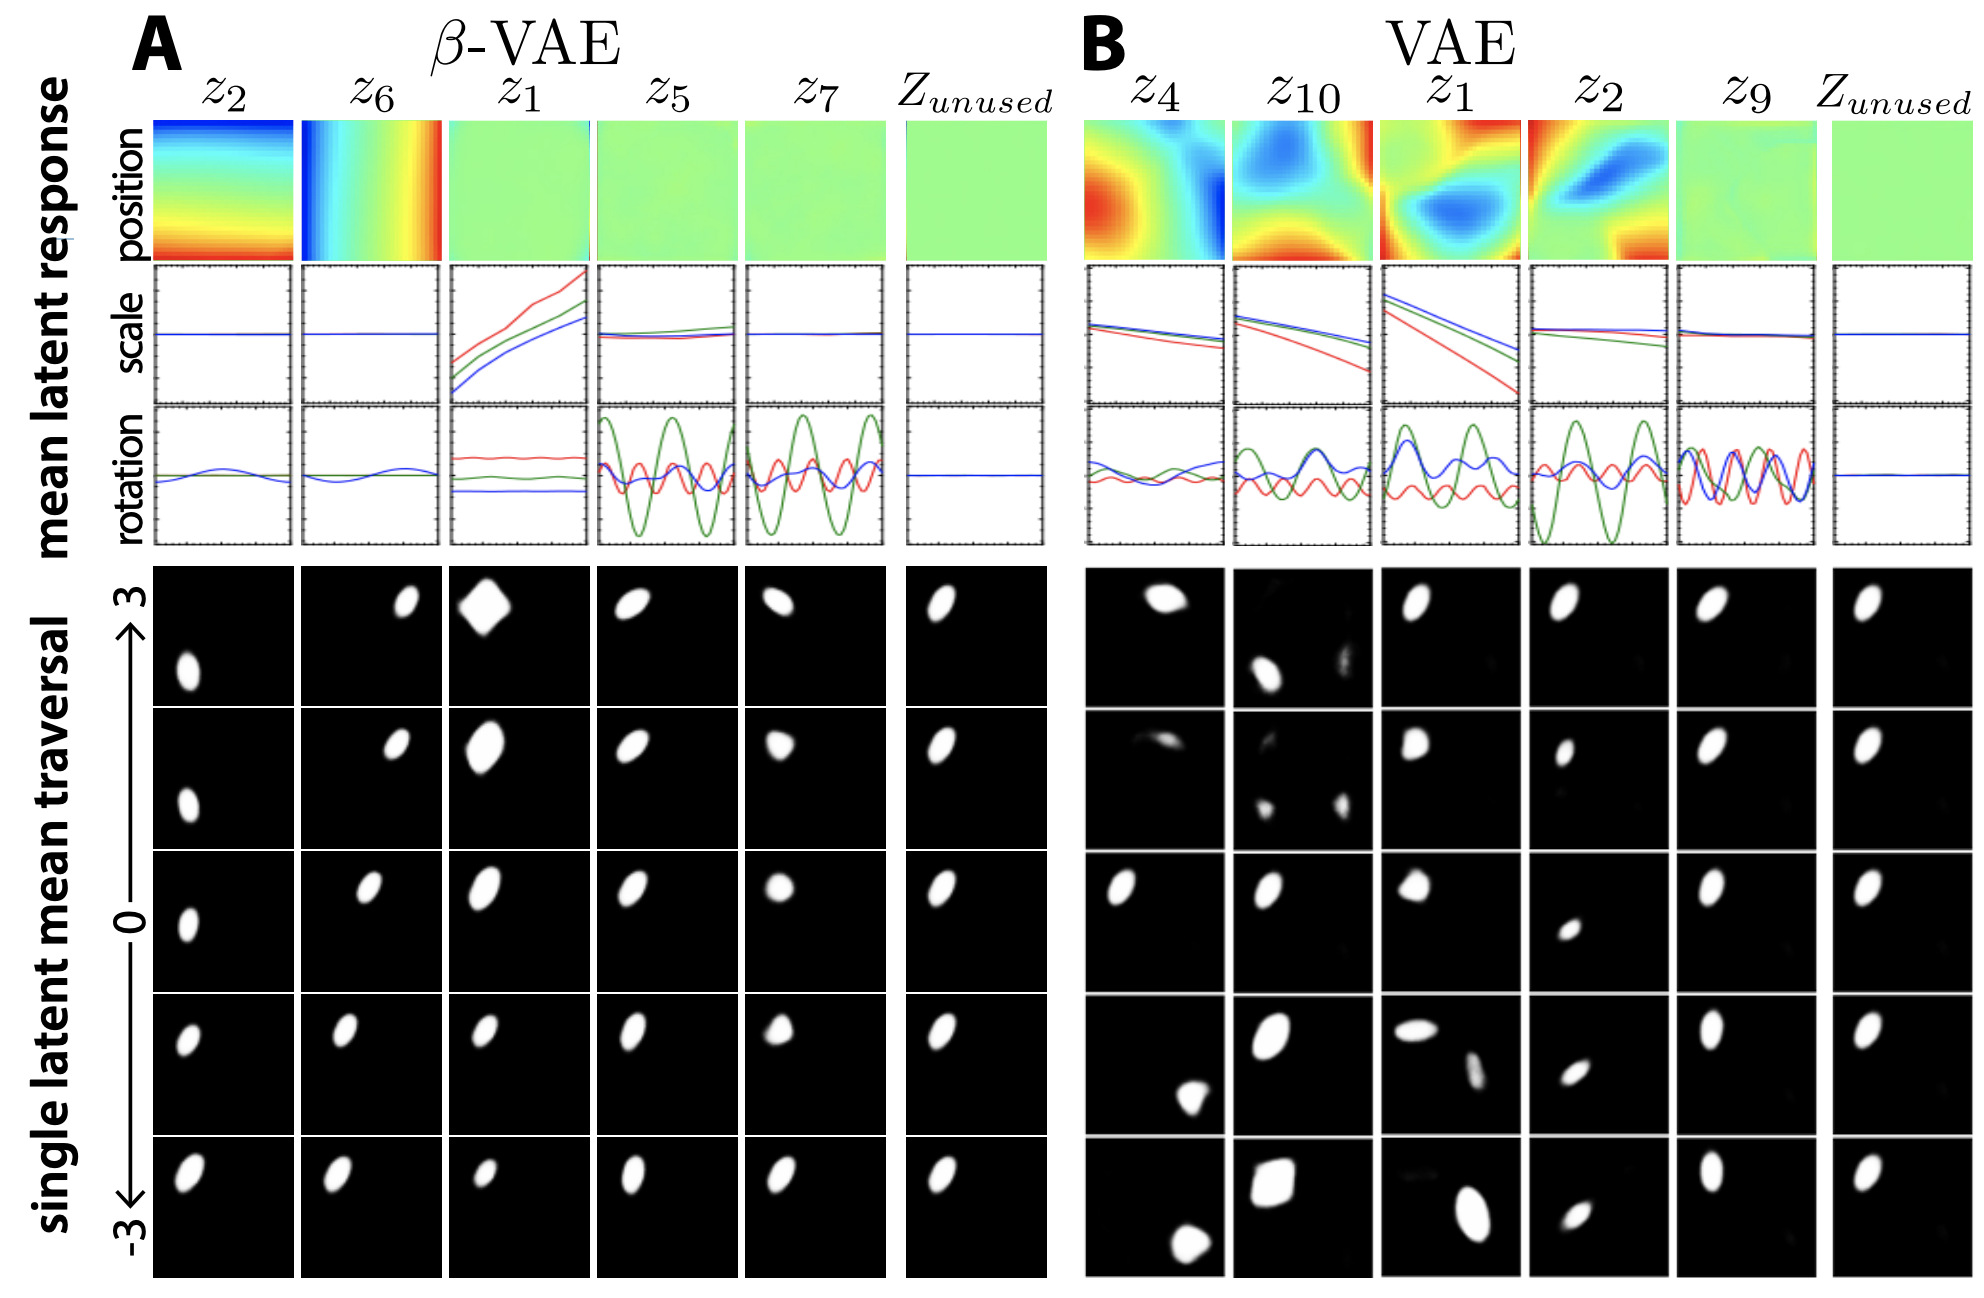
\includegraphics[width=.9\linewidth]{figs/betaVAE_5.png}
		\end{figure}

	\myfootnotewithlink{https://openreview.net/references/pdf?id=Sy2fzU9gl}{Higgins I. et al. beta-VAE: Learning Basic Visual Concepts with a Constrained Variational Framework, 2017}
\end{frame}
%=======
\begin{frame}{$\beta$-VAE}
	\begin{block}{ELBO}
		\vspace{-0.2cm}
		\[
		\mathcal{L}(q, \btheta, \beta) = \mathbb{E}_{q(\bz | \bx)} \log p(\bx | \bz, \btheta) - \beta \cdot KL(q(\bz | \bx) || p(\bz)).
		\]
		\vspace{-0.4cm}
	\end{block}
	\begin{block}{ELBO surgery}
		\vspace{-0.3cm}
		{\footnotesize
			\[
			\frac{1}{n} \sum_{i=1}^n \cL_i(q, \btheta, \beta) = \underbrace{\frac{1}{n} \sum_{i=1}^n \mathbb{E}_{q(\bz | \bx_i)} \log p(\bx_i | \bz, \btheta)}_{\text{Reconstruction loss}} - \beta \cdot \underbrace{\bbI_{q} [\bx, \bz]\vphantom{\sum_{i=1}}}_{\text{MI}} - \beta \cdot \underbrace{KL(q(\bz) || p(\bz))\vphantom{\sum_{i=1}}}_{\text{Marginal KL}}
			\]}
	\end{block}
	\begin{block}{Minimization of MI}
	\begin{itemize}
		\item It is not necessary and not desirable for disentanglement. 
		\item It hurts reconstruction.
	\end{itemize}
	\end{block}
	\myfootnotewithlink{https://arxiv.org/abs/1804.03599}{Burgess C. P. et al. Understanding disentangling in $\beta$-VAE, 2018}
\end{frame}
%=======
\begin{frame}{Summary}
\begin{itemize}
	\item Uniform dequantization is the simplest form of dequantization. 
	\vfill
	\item Variational dequantization is a more natural type that was proposed in Flow++ model.
	\vfill
	\item Disentanglement learning tries to make latent components more informative.
	\vfill
	\item $\beta$-VAE makes the latent components more independent, but the reconstructions get poorer.
\end{itemize}
\end{frame}
\end{document} 